\clearpage

\section{Superconducting circuit quantum devices}
In this part, we briefly discuss quantum information, then the quantum mechanics used in qubit manipulation and readout. Furthermore, the LC circuit, transmon, and gatemon physics are demonstrated.
 
I'm going to briefly introduce some quantum mechanics here to offer a better understanding of the later content. Let's begin with the most well-known time-dependent Schrödinger equation:
\begin{equation}\label{Scho-eq}
    i\hbar \frac{\partial \Psi}{\partial t} = \mathbf{H}\Psi = (-\frac{\hbar^2}{2m}\mathbf{\nabla}^2 + \mathbf{V})\Psi
\end{equation}
Where the left part is the Hamiltonian, the right is kinetic energy and potential energy operator. If we only treat the time evolution part, we get:
\begin{equation}\label{Time-evo}
    \Psi(t) = exp[-\frac{i}{\hbar}\int \mathbf{H}dt]\Psi(0) = \mathbf{U}(t)\Psi(0)
\end{equation}
Where $\mathbf{U}(t)$ is the time evolution operator. This equation shows that even though our Hamiltonian is time independent, our wave function is still rotating ceaselessly.

Traditionally we use the first-quantized wave function:
\begin{equation}
    \Psi[\mathbf{r_i}] = \prod_{i=1}^{N}\psi_{\alpha_i}(\mathbf{r}_i) \equiv \psi_{\alpha_1} \otimes \psi_{\alpha_2}\otimes ... \otimes \psi_{\alpha_N}  
\end{equation}
that is the direct product of all the individual wave functions in Hilbert space to calculate the total wave function. However, it would be more concise to use second quantization in the future quantum technology study. Instead of asking the state of each particle, we seek the number of particles in each state, which is the Fock state:
\begin{equation}
    |\Psi\rangle = |n_1, n_2, ..., n_k, ...\rangle, \sum n_k\equiv N
\end{equation}

N is the total number of particles. We can more easily calculate the hamiltonian of the system in this way. Moreover, it provides an intuitive way for people to understand the composition and evolution of the system.


% where $\sigma_i$ are Pauli matrices. Combined Eq.\ref{Time-evo}, we get:
% \begin{equation}
%     \mathbf{U}(t) = (\cos(\frac{|\mathbf{n}|}{\hbar}t)\sigma_0 - i \sin(\frac{|\mathbf{n}|}{\hbar}t)\hat{n} \cdot \overrightarrow{\sigma})
% \end{equation}

\subsection{Transmon}
\subsubsection{Quantum harmonic oscillator}
Suppose we have a capacitor C and an inductor L that are connected. By Kirchhoff's law, their voltage should be the same:
\begin{equation}
    V_C + V_L = 0
\end{equation}
Therefore, we can write the equation of motion for magnetic flux in the inductor and the charge on the capacitor as
\begin{equation}
\dot{Q} = -\Phi / L,\hspace{15}  \dot{\Phi} = Q / C
\end{equation}
which endows a frequency $\mathrm{\omega\textsubscript{0} = 1/\sqrt{LC}}$. Note that in normal metal without the superconducting state, this frequency is actually the collective movements of electrons. Still, there are many degrees of freedom for phonon and electron states. Recall that the energy stored in the capacitor and inductor is:
\begin{equation}
    T_C = \frac{Q^2}{2C} = \frac{C\dot{\Phi}^2}{2},\hspace{15} V_L = \frac{LI^2}{2} = \frac{{\Phi}^2}{2L}
\end{equation}
where $T_C$, $U_L$ corresponds to the kinetic energy and the potential energy. Now the Lagrangian of LC circuit in flux basis is:
\begin{equation}
    L = \frac{C\dot{\Phi}^2}{2} - \frac{{\Phi}^2}{2L}
\end{equation}
and hamiltonian is:
\begin{equation}
    H = \frac{Q^2}{2C} + \frac{\Phi^2}{2L}
\end{equation}
end of classical derivation.

To start dealing with the quantum world, we first check if the charge and flux coordinates can be propagated to operators by the Poisson bracket:
\begin{equation}
    \{\Phi, Q\} = \frac{\delta\Phi}{\delta\Phi}\frac{\delta Q}{\delta Q} - \frac{\delta Q}{\delta \Phi}\frac{\delta \Phi}{\delta Q} = 1
\end{equation}
Therefore, we can endow the two canonical variables with the commutator\cite{RN3}:
\begin{equation}
    \begin{array}{l}
    \Phi \to \hat\Phi \\
    Q \to \hat Q \\
    \, [ \hat\Phi, \hat Q ]  = i\hbar
    \end{array}
\end{equation}
which enables us to quantize the circuit:
\begin{equation}
    \mathbf{H} = \hbar\omega(a^\dagger a + \frac{1}{2})
\end{equation}
by using
\begin{equation}\label{chargeladder}
\begin{array}{cc}
     &   [a, a^\dagger] = 1, \\
     & \hat{\Phi} = \sqrt{\frac{\hbar Z}{2}}(a + a^\dagger), \\
     &  \hat{Q} = -i\sqrt{\frac{\hbar}{2Z}}(a - a^\dagger)
\end{array}
\end{equation}
where resonant frequency and impedance are respectively 
\begin{equation}
    \begin{array}{cc}
         &  \omega = \sqrt{\frac{1}{LC}},\\
         &  Z = \sqrt{\frac{L}{C}}
    \end{array}
\end{equation}

\begin{figure}[h!]
    \centering
    \includegraphics[width=0.4\textwidth]{Pic/QHO.png}
    \caption{The energy levels inside the potential well. The lowest level it can reach is $1/2\hbar\omega$.}
    \label{fig:my_label}
\end{figure}

So now we get an oscillator with evenly split energy levels. However, to utilize it in quantum computing, the system needs anharmonicity to avoid energizing particles to levels other than the ground and first excited state. Many attempts\cite{RN18, RN19, RN20} such as charge qubits, phase qubits, and flux qubits are demonstrated. None of them are strictly two-level system, but they all exhibit protections of two-level subspace. We describe these circuits as artificial atoms in the circuit quantum electrodynamics (circuit QED or cQED)\cite{RN15, RN1, RN8}. In the following content, charge qubits, mostly transmon, will be the central part.

\subsubsection{Josephson junction}
Suppose we are BCS superconductor\cite{RN36}, then we introduce new basis $\Hat{n} = \hat{Q}/2e$, $\hat{\phi} = {2\pi \hat{\Phi}} / {\Phi_0}$, where $\Phi_0$ is the magnetic flux quanta. If we sandwiched a thin insulator, like aluminum oxide, between two superconductors, we can get a Josephson junction (JJ). The current phase relation (CPR) of JJ is described as\cite{RN14}:
\begin{equation}
I = I_0\sin{\phi}    
\end{equation}
This is known as DC Josephson effect. If we apply a voltage across the junction, the phase difference will evolve:
\begin{equation}
    \frac{d\phi}{dt} = \frac{2eU}{\hbar}
\end{equation}
which is AC Josephson effect, with Josephson frequency $f_J = 483.6 GHz \cdot  U/ mV$. These relations give Josephson junctions with non-linear inductance
\begin{equation}
L(\phi) = \frac{\Phi_0}{2\pi I_0 \cos{\phi}}    
\end{equation}, which is crucial for the anharmonicity in superconducting qubits.

To draw out the current-voltage characteristics of JJs, we consider a simple model called resistively and capacitively shunted junction (RCSJ)\cite{RN35}. The JJs now transform into a circuit composed of JJ, resistor, capacitor, thermal noise generator, and voltage source. Here through Kirchoff's law, we get:
\begin{equation}
    I + I_N(t) = I_0 \sin{\delta} + \frac{U}{R} + C\dot{U}.
\end{equation}
\begin{figure}[h!]
    \centering
    \includegraphics[width=0.7\textwidth]{Pic/RSCJ_circuit.png}
    \caption{The equivalent circuit for RCSJ model. The circuit components from left to right are: Josephson junction, resistor, thermal noise generator and capacitor.}
    \label{fig:my_label}
\end{figure}
Replace voltage with AC Josephson effect:
\begin{equation}
    I + I_N(t) = I_0 \sin{\delta} + \frac{\Phi_0}{2\pi R}\dot{\delta} + \frac{\Phi_0 C}{2\pi}\Ddot{\delta} 
\end{equation}. 
Change time $t$ to Josephson time constance $\tau = t\omega_c$ with characteristic frequency $\omega_C = \frac{2\pi}{\Phi_0}I_0 R$, the equation of motion eventually becomes:
\begin{equation}
    \beta_C \Ddot{\delta} + \dot{\delta} + \sin{\delta} = \frac{I}{I_0} + \frac{I_N}{I_0}
\end{equation}
with Stewart-McCumber parameter $\beta_C = \frac{2\pi}{\Phi_0}R^2 C$. While the system is overdamped with $\beta_C \ll 1$, the system is not hysteresis. Namely, the critical current and the retrapping current are the same, and vice versa. The JJs used in our experiment are mostly underdamped then hysteresis with retrapping current $\frac{I_r}{I_0} \approx\frac{4}{\pi}\frac{1}{\sqrt{\beta_c}}$, therefore while searching for the critical current of JJs, we usually scan from superconducting state to normal state.

\subsubsection{Charge qubit}
In many experiments, the JJs are superconductor-insulator-superconductor (SIS) junctions. We replace the linear inductor term and get the Hamiltonian\cite{RN7}:
\begin{equation}\label{HamiltonianCharge}
    \hat{H} = 4E_C (\hat{n} - n_g)^2 - E_J \cos \hat{\phi}
\end{equation}
where 
\begin{equation}\label{JJenergy}
    E_J = \Phi_0 I_c / 2\pi 
\end{equation}
is the Josephson energy, $E_c = e^2 / 2(C_g + C_J)$ is the charging energy and $n_g = Q_r / 2e + C_g V_g /2e$, as $Q_r$ the charge in the environment. 
In the extreme of $E_C \gg E_J$, we can create a Cooper Pair Box (CPB), namely, charge qubit. After numerically solving, diagonalizing in charge basis, charge qubit can be intuitively imaged by its hamiltonian:
\begin{equation}\label{CPB_H}
    \hat{H} = 4E_C\sum_N (\hat{n} - n_g)^2|N\rangle \langle N| - \frac{1}{2} E_J \sum_N (|N\rangle\langle N+1| + |N+1\rangle \langle N |)
\end{equation}
, where N is the number of Cooper pairs inside the island. The energy band is shown below (Fig \ref{Transmon_e}). Notice that when $N_g = 0$, if we have $N=0$, we are in $|0\rangle$, ground state, and same for 1. When we slowly charge the island to N = 1/2, we can get $|+\rangle = \frac{1}{\sqrt{2}}(|0\rangle + |1\rangle)$. Although the mechanics look easy, the realization of it is hard since the environment is perturbing the system all the time, causing decoherence.
\begin{figure}[h!]
\captionsetup[subfigure]{labelformat=empty}
    \centering
    \begin{subfigure}[b]{0.48\textwidth}
         \centering
         \includegraphics[ width=1\linewidth]{Pic/Transmon_elevel_1.png}
         \caption{}
         \label{TaNWonchip}
     \end{subfigure}
     \hfill
     \begin{subfigure}[b]{0.48\textwidth}
         \centering \includegraphics[width=1\linewidth]{Pic/Transmon_elevel_5.png}
         \caption{}
         \label{fig:three sin x}
     \end{subfigure}
    \begin{subfigure}[b]{0.48\textwidth}
         \centering \includegraphics[width=1\linewidth]{Pic/Transmon_elevel_10.png}
         \caption{}
         \label{fig:three sin x}
     \end{subfigure}
     \hfill
     \begin{subfigure}[b]{0.48\textwidth}
         \centering \includegraphics[width=1\linewidth]{Pic/Transmon_elevel_50.png}
         \caption{}
         \label{fig:three sin x}
     \end{subfigure}

    \caption{The energy level of transmon respect to different $E_J / E_C$. The x-axis is the total Cooper pairs number in the qubit island. Notice that the energy is less sensitive to charge when $E_J / E_C$ becomes larger}
    \label{Transmon_e}
\end{figure}

\subsubsection{Transmon}
To reach the goal of mitigating the charge noise, people try to engineer the charge-Josephson energy relationship in the CPB, flattening the potential on each level. Here transmon, that is, transmission line shunted plasma oscillation qubit, comes out and immediately becomes popular in many laboratories.\cite{RN6, RN13}

\begin{figure}[h!]
    \centering
    \includegraphics[width=0.5\linewidth]{Pic/QHO_transmon.png}
    \caption{The cosine potential well, along with the energy level of transmon. The excitation energy $\hbar\omega_{1\shortrightarrow 2}$, $\hbar\omega_{2\shortrightarrow 3}$ are calculated according to Eq \ref{TransmonQHO}. Nonlinearity gives a different transition frequency between levels and therefore protects the qubits in the ground and first excited subspace.}
    \label{fig:my_label}
\end{figure}

Now, the system is in a different regime, where $E_J \gg E_c$, the charge sensitivity is suppressed, and anharmonicity is still maintained. Neglect the charge offset and do Maclaurin expansion on Eq.\ref{CPB_H}, we get transmon Hamiltonian:
\begin{equation}
    \mathbf{H} = 4E_C\hat{n}^2 - E_J + \frac{E_J\hat{\phi}^2}{2} - \frac{E_J\hat{\phi}^4}{24} +  \mathcal{O}(\hat{\phi}^6).
\end{equation}
with eigenenergies:
\begin{equation}\label{TransmonQHO}
    E_m \simeq -E_J + \sqrt{8E_C E_J}(m+\frac{1}{2}) - \frac{E_C}{12}(6m^2 + 6m + 3).
\end{equation}
Notice that the negative quadratic term offers $\alpha = \omega^{1\to 2}_q - \omega^{0\to 1}_q = -E_C$, the system's anharmonicity, a negative number around 100 - 300 MHz in transmon. The desirable operating transmon qubit frequency is 3 - 6 GHz.

To tune the frequency of transmon, we can introduce a parallel Josephson junction circuit instead of a single Josephson junction and apply a magnetic field in the loop. This technique is also called superconducting quantum interference device (SQUID) and can be used in detecting an extremely subtle magnetic field. The theory behind the SQUID is the integer number of superconducting flux quanta equals the sum of all the phase components across the Josephson junctions, that is:
\begin{equation}\label{SQUIDflux}
    \phi_1 - \phi_2 + \phi_e = 2\pi k
\end{equation}
. Rewriting the Hamiltonian of Josephson junction into\cite{RN6}:
\begin{equation}\label{SQUIDEj}
    \hat{H}_J = -E_{J1}\cos{\hat{\phi}_1} -E_{J2}\cos{\hat{\phi}_2}
\end{equation}
, and then combine Eq \ref{SQUIDflux} and Eq \ref{SQUIDEj}, we get the Josephson junction Hamiltonian:
\begin{equation}
    \hat{H}_J = -E_{J\Sigma}\cos{ \left( \frac{\pi \Phi}{\Phi_0} \right) } \sqrt{1+d^2\tan^2\left( \frac{\pi\Phi}{\Phi_0}\right)}\cos{(\hat\varphi - \varphi_0)}
\end{equation}
, where $\varphi = (\phi_1 + \phi_2) / 2$ and $E_{J\Sigma} = E_{J1} + E_{J2}$. The effective Josephson energy can write as:
\begin{equation}
    E_{J\text{eff}} = -E_{J\Sigma}\cos{ \left( \frac{\pi \Phi}{\Phi_0} \right) } \sqrt{1+d^2\tan^2\left( \frac{\pi\Phi}{\Phi_0}\right)}
\end{equation}
. Now we get a similar Josephson energy formula to the normal transmon one, and we can utilize this external field to gain more degree of freedoms in qubit.
\begin{figure}[h!]
    \centering
    \includegraphics[width=0.5\textwidth]{Pic/Fluxmon.png}
    \caption{A flux tunable transmon with symmetric Josephson junction. The magnetic field is usually generated from a flux line close to the SQUID.}
    \label{fig:my_label}
\end{figure}



\subsection{Gatemon}

The previous section introduces frequency tunable transmon through magnetic flux, which idea is crucial in quantum computing since we can use it to do fast gate operations and reduce frequency-dependent noise\cite{RN29}. However, this system has downsides like heat dissipation from the current flowing through the flux line, the crosstalk among qubits, and flux noises\cite{RN28}. To eliminate these downsides, we introduce a new system called gatemon, also known as semiconductor gate tunable transmon\cite{RN73}.
\subsubsection{Proximitized effect}
Imagine a normal metal that is connected by superconductors on both sides. Since it is the cooper pairs that are conducting in the BCS superconductor, when they enter the normal metal, it remains 'pairs' because of the non-locality of particles as long as the characteristic length is longer than the connection\cite{RN32}. This effect is called proximitized effect, and it is used in nowadays' quantum device\cite{RN33}. To gain control of this effect, we can use a semiconductor as the connection and implement a nearby gate. By tuning the gate voltage, the bare semiconductor will feel a large electric field and reduce its conductivity channels. In the extreme case, we can completely pinch off the semiconductor, making it act as an infinity resistance component. There are several ways of realizing the tunable connection, such as 2-dimensional electron gas (2DEG), and semiconductor-superconductor hybrid nanowire with S-N-S junction.

\subsubsection{Andreev reflection}
The detailed mesoscopic explanation of the boundary of the N-S surface for this effect is described by Andreev Reflections. There are two branches of excitations in semiconductor, electron with charge $-e$, momentum $\mathbf{p}$, and group velocity $\mathbf{v_p}$, and holes with charge $e$ and group velocity $\mathbf{\bar{v}_p} = -\mathbf{v_p}$. In N-I surface, the electron will experience specular reflection, endow the outgoing electron $\mathbf{p'} = \mathbf{p} - 2\hat{\mathbf{n}}(\hat{\mathbf{n}}\cdot\mathbf{p})$. However, for the N-S interface, the electrons undergo the retro reflection, generate holes with opposite momentum and shoot Cooper pairs into the superconductor subgap. Due to the impurities and defects that exist on the interface, there is still a finite probability that the electrons reflect specularly, resulting in an imbalance charge transfer between leads.
\begin{figure}[h!]
    \centering
    \begin{subfigure}[b]{0.45\textwidth}
         \centering
         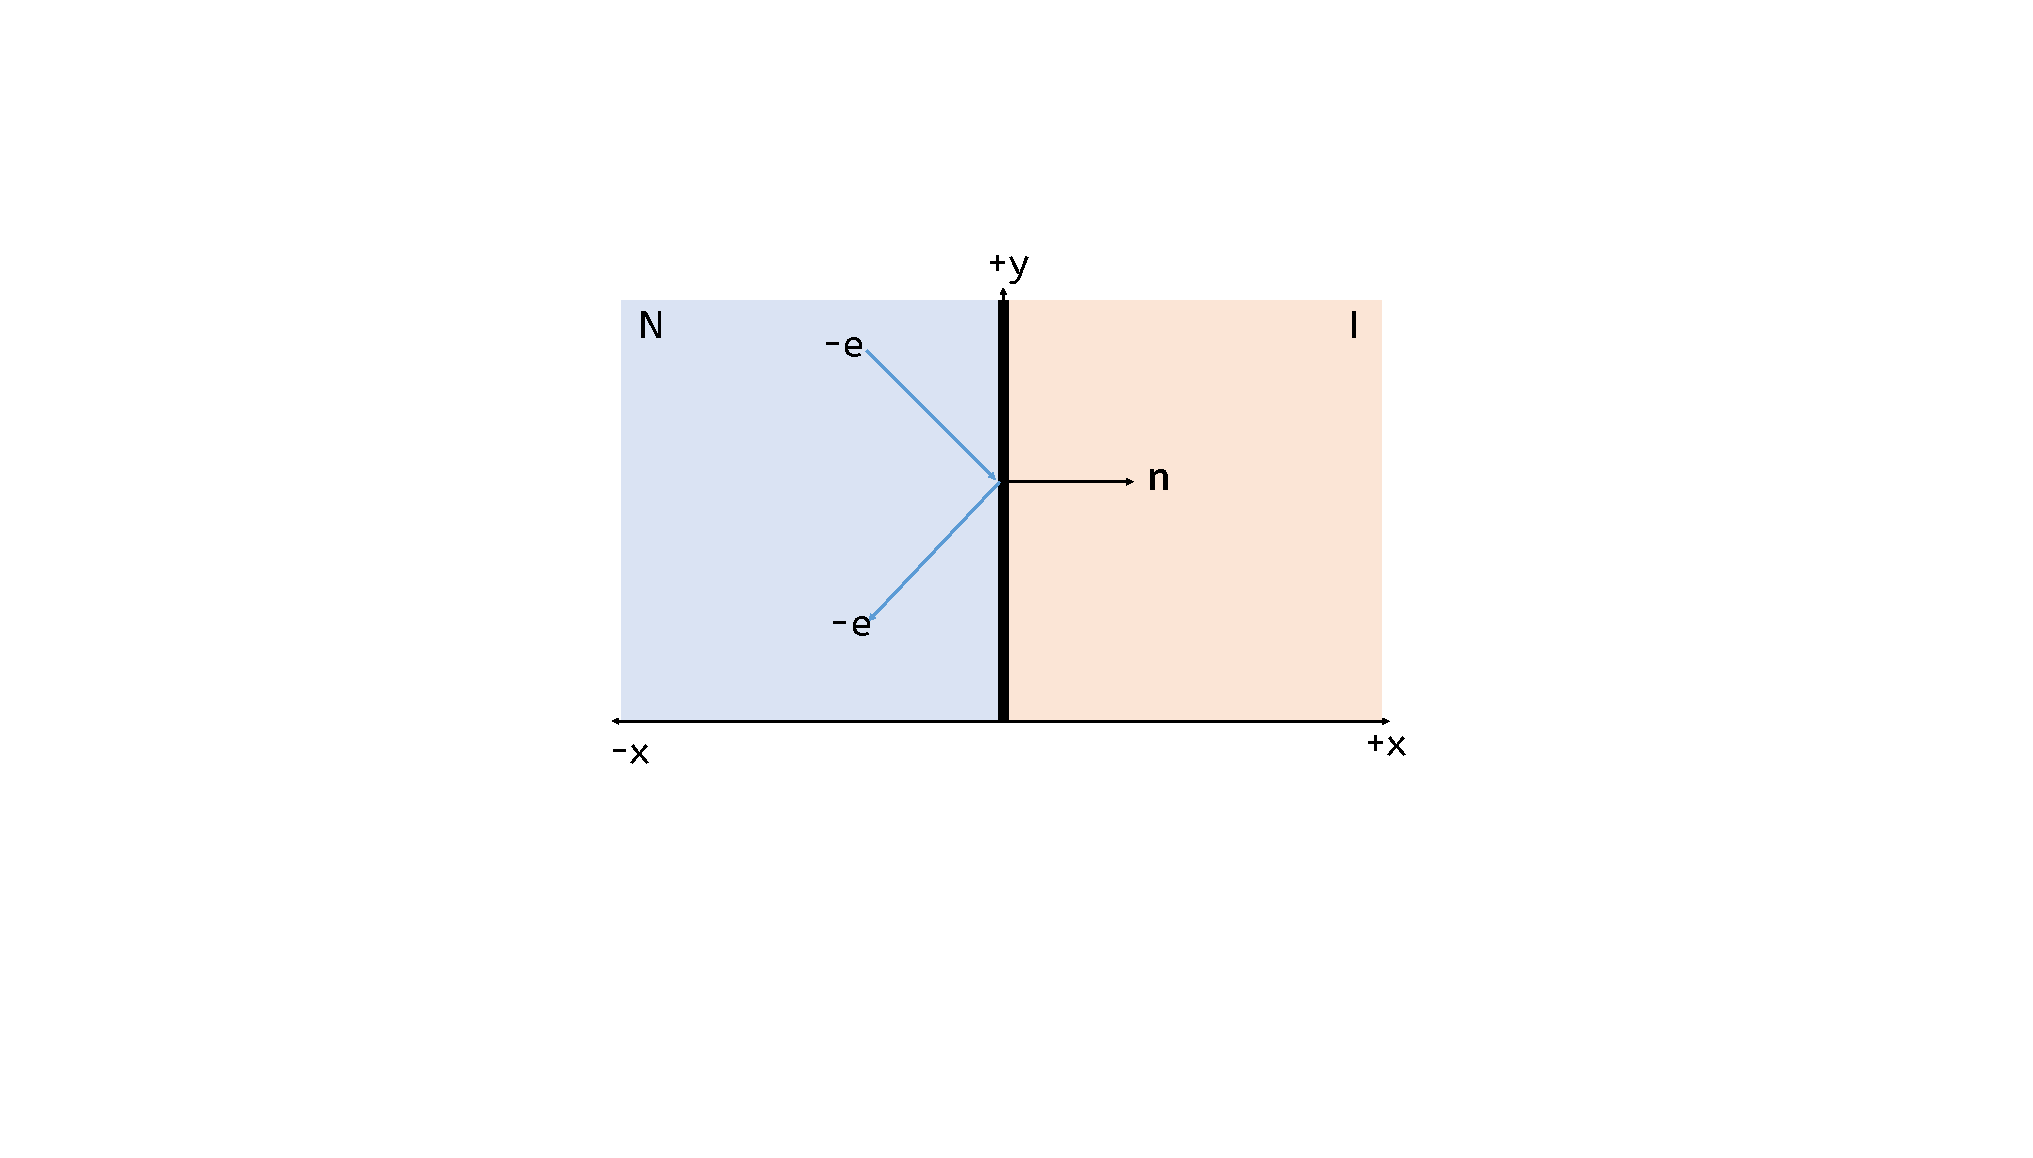
\includegraphics[trim={10cm 5.8cm 4.5cm 3.5cm},clip, width=1.5\linewidth]{Vec_Pic/AndreevReflectionNI.eps}
         \caption{}
         \label{TaNWonchip}
     \end{subfigure}
     \hfill
     \begin{subfigure}[b]{0.45\textwidth}
         \centering
         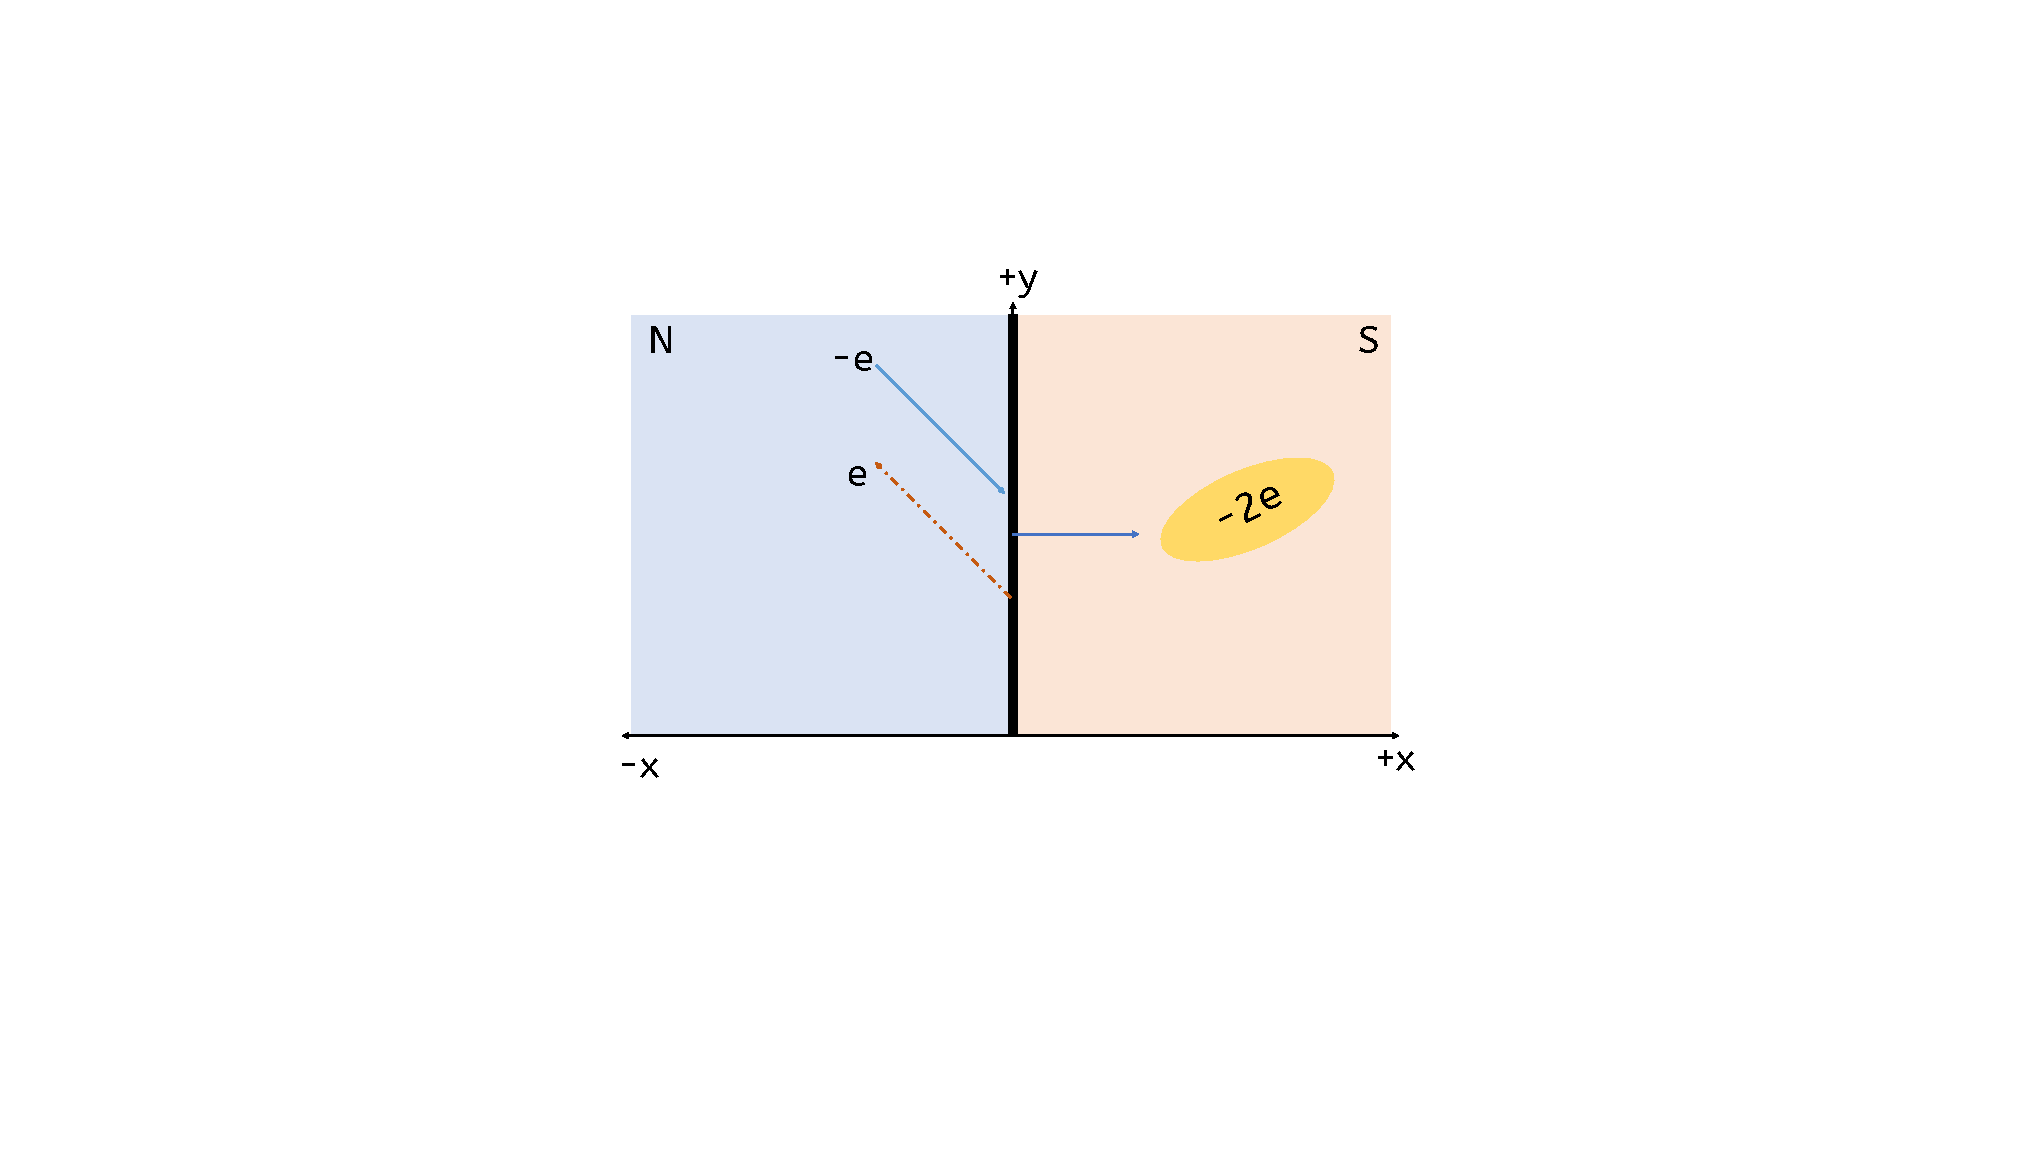
\includegraphics[trim={10cm 5.5cm 4cm 3.5cm},clip, width=1.5\linewidth]{Vec_Pic/AndreevReflection.eps}
         \caption{}
         \label{fig:three sin x}
     \end{subfigure}
    \caption{(a) Specular reflection with no generation of quasi-particles at the normal metal (semiconductor) -insulator (NI) interface. $\mathbf{n}$ is the normal vector of the interface (b) Andreev reflection with the generation of Cooper pair inside the superconductor}
    \label{AR}
\end{figure}

N-S interface was theoretically discussed in the 1970s but did not gain attention until decades later\cite{RN31, RN30}. One important model for describing metallic to tunneling regime transition on semiconductor is introduced by Blonder, Tinkham, and Klapwijk (BTK) theory\cite{RN31}, which introduces a barrier strength Z to quantitatively indicate the number of impurities and defects on the boundary. We write the plane wave solution of particle as $|k_0\rangle = \begin{pmatrix}
  u_0\\ 
  v_0
\end{pmatrix}e^{ikr}$, as $u_0$ and $v_0$ are coherence factors of electrons and holes, and get the propagating wave in the semiconductor:
\begin{equation}
    \Psi_N(r) = \begin{pmatrix}
  1\\ 
  0
\end{pmatrix}e^{ik_n^+r}+A(E)
\begin{pmatrix}
  0\\ 
  1
\end{pmatrix}e^{ik_n^-r}+B(E)
\begin{pmatrix}
  1\\ 
  0
\end{pmatrix}e^{-ik_n^+r}
\end{equation}
, where A and B are probability amplitudes of Andreev reflection and specular reflection. Similarly, in the superconductor, we have:
\begin{equation}
    \Psi_S(r) = C(E)
\begin{pmatrix}
  u_0\\ 
  v_0
\end{pmatrix}e^{ik_s^+r}+D(E)
\begin{pmatrix}
  u_0\\ 
  v_0
\end{pmatrix}e^{-ik_s^-r}
\end{equation}
, which describes the transmission of electrons without and with branch crossing. By the number conservation of particles, there must be:
\begin{equation}
    A(E) + B(E) + C(E) + D(E) = 1
\end{equation}
\begin{figure}[htbp]
    \centering
    \includegraphics[width=0.6\linewidth]{Pic/BTK_theory.jpg}
    \caption{The BTK theory model schematic. The normal metal electrons (blue) on the left side undergo Andreev reflections and specular reflections. The quasi-particles (holes and electrons) are formed on the superconductor side. The superscript + and - on $k$ means electrons and holes}
    \label{BTKtheorypic}
\end{figure}
and we get the general form of solution:
\begin{equation}
    |A| = \left\{
    \begin{array}{ll}
        \frac{\Delta^2}{E^2+(\Delta^2 - E^2)(1+2Z^2)^2}  & \text{for } E < \Delta \\
        \frac{u_0^2 v_0^2}{\gamma^2} & \text{for } E > \Delta
    \end{array},
    |B| = \left\{
    \begin{array}{ll}
       1 - |A|^2 & \text{for } E < \Delta\\
        \frac{(u_0^2 - v_0^2)^2 Z^2 (1+Z^2)}{\gamma^2}  & \text{for } E > \Delta
    \end{array}
\end{equation}
where $\gamma^2 = [u_0^2 + Z^2(u_0^2-v_0^2)]^2$, and $u_0^2 = 1-v_0^2 = \frac{1}{2}\{ 1+[(E^2 - \Delta^2)/E^2]^{\frac{1}{2}}\}$. Since the transmission rate at N-S interfaces below the superconducting gap is 0 ($C(E) = D(E) = 0$), we can then utilize these solutions to find current:
\begin{equation}
    I_{NS} = \frac{2e}{h}\int [f(E-eV)][1+A(E)-B(E)]d
\end{equation}
with $f$ the Fermi-Dirac distribution functions and V the bias voltage across the interface. Overall, we can say that Andreev reflections describe the cooper pairs breaking into electron-hole pairs inside the semiconductor, then creating non-conventional superconductivity\cite{RN10}.

\subsubsection{Multiple Andreev Reflection}
\begin{figure}[h!]
    \centering
    \includegraphics[width=0.6\textwidth]{Pic/MARs.png}
    \caption{The demonstration of multiple Andreev reflections of order 3. The x-axis is spacial distance and y-axis is electron energy.}
    \label{fig:my_label}
\end{figure}
A phenomenon emerges when two N-S interfaces are encapsulated between two superconducting leads on a small scale. Electrons in semiconductors first hit the N-S interface through Andreev reflection, creating a hole that bounces back. The hole again hits the other N-S interface and bounces back. This process with multiple bounces is called Multiple Andreev Reflection (MAR), with orders $n+1$ where $n$ is the number of AR.

In this scenario, the threshold voltage can be represented as:
\begin{equation}
    V_{th} = \frac{2\Delta}{en}
\end{equation}
which can provide conductance peaks in the junctions' I-V characteristic. It's worth noticing that the MAR is observed only when the barrier strength Z is small and the transmission probability is high. Given the phase coherence between the two Andreev reflection processes, a subgap state, Andreev Bound State (ABS), is formed and can be readout through high-frequency measurement\cite{RN51}.

\subsubsection{Andreev bound state}
\begin{figure}[h!]
    \centering
    \includegraphics[width=0.6\textwidth]{Pic/ABS.png}
    \caption{The Andreev bound state happens inside the semiconductor.}
    \label{fig:my_label}
\end{figure}
Andreev bound state is the essential process that happens inside the semiconductor. The states are characterized by their transmission eigenvalues ${T_i}$\cite{RN78}. We can write the ground and excited state energy of the ABS as:
\begin{equation}
    E_{ABS}(T, \delta) = \mp \Delta \mathlarger{\sum}_i\sqrt{1-T_i\sin^2{\left(\hat{\delta}/2\right)}}
\end{equation}
\begin{figure}[h!]
    \centering
    \includegraphics[width=0.6\textwidth]{Pic/ABS_transmission.png}
    \caption{The ABS energy in phase space with different transmission rate. When the transmission is 1, the energy gap between the states is closed at $\phi = \pi$. }
    \label{fig:my_label}
\end{figure}

Then we use Taylor expansion on the ground state energy, substitute the result for the Josephson energy part in Eq \ref{HamiltonianCharge}, we can get the energy of each level in gatemon and the anharmonicity of the qubit with respect to the transmission rate (detail calculation is in Anders' PhD thesis\cite{RN79}):
\begin{equation}
    E_{12} - E_{01} = \alpha \approx -E_C \left(1-\frac{3\sum T_i^2}{4\sum T_i}\right)
\end{equation}.

Therefore, with the S-Sm-S junction, the anharmonicity changes and it is related to the transparency of the N-S interface and the mean-free path of the electrons inside the junction.  

\subsection{Circuit QED readout and qubit control}
\subsubsection{Circuit-QED readout}
Superconducting qubits usually need an auxiliary readout solution to obtain the system's state. Several readout strategies exist, like a SQUID as a sensitive magnetic flux detector and a single electron transistor as a sensitive charge detector. The qubit in our system is read out by coupling to a readout resonator, a harmonic oscillator system.

We can write a qubit transverse coupling to a resonator as following\cite{RN8}:
\begin{equation}
    H = \omega_ra^\dagger a-\frac{\omega_q}{2}\sigma_z + g(\sigma^-a^\dagger+\sigma^+a)
\end{equation}
, with $g$ the coupling strength. The terms in the hamiltonian are resonator energy, qubit energy, and interaction. This formula is the well-known Jaynes-Cumming model, which describes the interaction between an opti0cal field and a two-level system. If the qubit and resonator frequency detune significantly compared to the coupling strength, that is $\lambda = g / \Delta \ll 1$ with $\Delta = \omega_q-\omega_r$, the system is in dispersive regime. We introduce a unitary transformation operator 
\begin{equation}
    U = \exp[{\lambda(\sigma^-a -\sigma^-a^\dagger)}]
\end{equation}
and then the hamiltonian:
\begin{equation}
    H_D = U_DH_DU_D^\dagger \approx (\omega_r-\chi\sigma_z)a^\dagger a-\frac{\omega_q+\chi}{2}\sigma_z
\end{equation}
, here $\chi = g^2 / \Delta$ is the dispersive shift. The hamiltonian tells us the resonator frequency will change by $2\chi$ depending on the qubit state. Rewrite the Hamiltonian with terms in different basis:
\begin{equation}\label{TLSresonatorH}
    H_D = \omega_r a^\dagger a - \frac{1}{2}(\omega_q + \frac{g^2}{\Delta} + \frac{2g^2}{\Delta}a^\dagger a)\sigma_z
\end{equation}
. The additional $2g^2/\Delta$ term is called ac-Stark shift. This effect has resulted in photon number fluctuations leading to shifts in qubit frequency, thus dephasing. 

We now have a circuit-QED-based gatemon qubit, and we want to read out and manipulate it through the co-planar waveguide, the on-chip circuit. From Eq \ref{TLSresonatorH} we already know how the readout system generally works. The circuit-QED into the resonator coupled system is described in Hamiltonian\cite{RN6}:
\begin{equation}
    H = 4E_C(\hat{n} - n_g)^2 - E_J\cos{\hat{\phi}} + \hbar\omega_r a^\dagger a + 2\beta V^0_{rms}\hat{n}(a + a^\dagger)
\end{equation}
, where $\beta = C_g/C_\Sigma$, with $C_\Sigma$ the total capacitance to the ground and $C_g$ the resonator qubit coupling capacitance, and $V^0_{rms} = \sqrt{\hbar\omega_r / 2C_r}$ the rms voltage of resonator. The final derivation after second quantization is the same as \ref{TLSresonatorH}, but with $g = 2\beta e V^0_{rms}$.

\subsubsection{Qubit control}
Now assume we have prepared a two-level system, and our target is to investigate how the system evolves under external control source\cite{RN11}. Suppose we use a microwave as the external control field:
\begin{equation}
\lambda (t) = E(t) \cos{(\omega_d t + \xi(t))}    
\end{equation}
, where  $\xi(t)$ is an arbitrary time-dependent phase factor for anharmonic oscillation, the Hamiltonian under laboratory (Schrodinger) frame is:
\begin{equation}\label{lab_hamil}
    \mathbf{H}_L(t) = \sum_{n=0,1} \epsilon_n |n\rangle\langle n| + \hbar\lambda(t) (|0\rangle\langle 1| + |1\rangle\langle 0 |)
\end{equation}
, with the ground state energy $\epsilon_0 = -\hbar\omega_q/2$ and $\epsilon_1 = +\hbar\omega_q/2$ .
We then want the Dirac picture, namely rotation frame hamiltonian $\mathbf{H}_R$. Suppose we have a rotation operator $\mathbf{R}$, with $|\Psi ' (t)\rangle = \mathbf{R}|\Psi(t)\rangle$, combined with Eq.\ref{Scho-eq}:
\begin{equation}\label{Rota_frame}
    \mathbf{H_R'} = i\hbar \mathbf{\dot{R}{R^\dagger}} + \mathbf{RH_0{R^\dagger}}
\end{equation}
where $\mathbf{H_0}$ is the Hamiltonian of the state $|\Psi (t)\rangle$. The rotation operator can be formalized as:
\begin{equation}\label{rota_op}
    \mathbf{R}(t) = \exp\{ -i\sum_{n=0,1} (n-\frac{1}{2}) [\omega_d t + \phi (t)] |n\rangle\langle n|\}
\end{equation}
Plug Eq.\ref{lab_hamil} and Eq.\ref{rota_op} into Eq.\ref{Rota_frame}, and define a phase factor $\varphi (t) = \phi (t) - \xi (t)$, we obtain:
\begin{equation}\label{TLScontrolH}
    \mathbf{H}_R (t) = \frac{\hbar}{2}\mathbf{B}(t) \cdot \mathbf{\sigma}
\end{equation}
after rotating wave approximation (RWA). Here $\mathbf{B}(t) = (E(t)\cos{\varphi(t)}, E(t)\sin{\varphi(t)}, \dot\phi(t))$ is an effective external field, and $\sigma$ is the Pauli operator $(\sigma_x, \sigma_y, \sigma_z)$. The driving frequency $\omega_d$ is usually tuned to be the same as $\omega_{01}$.

Experimentally, we can treat the superconducting qubit as spin-$\frac{1}{2}$ particle and omit the constant energy term. By choosing the combination we needed in parameter space $(E(t), \phi (t), \varphi (t))$, we can manipulate the qubit freely.

Let's now focus on the qubit control on superconducting qubit. Consider an external drive source with signal $V_D$, the Lagrangian of the circuit with a harmonic oscillator (like a qubit):
\begin{equation}
    \mathcal{L} = \frac{1}{2}C_J\dot{\Phi}^2 + \frac{1}{2}C_d(\dot{\Phi} - V_d)^2 - \frac{\Phi^2}{2L}
\end{equation}
, where $C_d$ is the drive-qubit coupling capacitance. The charges of the system $Q = \frac{\partial \mathcal{L}}{\partial \dot{\Phi}} = (C_J+C_d)\dot{\Phi}$, and the Hamiltonian becomes:
\begin{equation}
    H = \frac{Q^2}{2(C+C_d)} + \frac{\Phi^2}{2L} + C_d V_d\dot{\Phi} - \frac{1}{2}C_d V_d^2
\end{equation}
. Generally, the coupling capacitance $C_d$ is far smaller than $C$. So omit the last constant term and let $C_\Sigma = C_J + C_d$, we get:
\begin{equation}
    H = \hbar\omega(a^\dagger a + \frac{1}{2}) - \frac{C_dV_d}{C_\Sigma}\sqrt{\frac{\hbar}{2Z_r}}\cdot i(\hat{a}^\dagger - a)
\end{equation}
In qubit, the Hamiltonian simplify to two levels:
\begin{equation}
    H_d = -\frac{1}{2}\hbar \omega_q \sigma_z + \Omega V_d\sigma_y
\end{equation}
with $\Omega=\frac{C_dV_d}{C_\Sigma}\sqrt{\frac{\hbar}{2Z_r}}$. In rotation frame (Eq.\ref{Rota_frame}) with the time evolution operator (Eq.\ref{Time-evo}), the Hamiltonian becomes:
\begin{equation}
    \tilde{H}_d = \Omega V_d(t) (\cos{(\omega_q t)}\sigma_y - \sin{(\omega_qt)}\sigma_x)
\end{equation}
Let $V_d(t) = V_0v(t)$, and with generic electromagnetic wave form:
\begin{equation}
    \begin{array}{rl}
         v(t) =& s(t)\sin{(\omega_dt+\phi})  \\
         =& s(t)(\cos{\phi}\sin{(\omega_dt)}+\sin{\phi}\cos{(\omega_dt)})
    \end{array}
\end{equation}
where $s(t)$ is a dimensionless envelop function. Use the definitions:
\begin{equation}
\begin{array}{rlr}
    I =&\cos{\phi} \hfill &\text{(In-phase component)}  \\
    Q =&\sin{\phi} \hfill &\text{(Out-of-phase component)}
\end{array}
\end{equation}
with RWA approximation and set drive frequency $\omega_d = \omega_q$, we get:
\begin{equation}
    \tilde{H}_d = -\frac{\Omega}{2}V_0s(t)(I\sigma_x+Q \sigma_y)
\end{equation}
The formula shows that the in-phase and out-of-phase pulse will rotate the qubit around the x-axis and the y-axis. For example, for an in-phase pulse, the time-evolution operator becomes:
\begin{equation}
    U(t) = \exp([\frac{i}{2}\Omega V_0\int^t_0s(t')dt']\sigma_x)
\end{equation}
By choosing the drive time, we can continuously drive the qubit around the x-axis. 


\subsection{Noise and decoherence}

One important factor that limits the coherence time and high fidelity manipulations of qubits is the noise. Since our device is cooled down to around 20 mK (approximately 1.72 $\mu$eV in thermal energy), and the qubit transition energy $f_{01} / h$ is $20\mu$eV at 5 GHz, the heat excitation generated by phonons and the $50\Omega$ resistors, namely Johnson noise is one minor source of white noise in the system. At this temperature and high frequency, Nyquist noise has a higher power density than Johnson noise, and it originates from the qubits' spontaneous emission to the environment. Another important noise is called $1/f$ noise with power spectrum density (PSD): $S(f) = 1/f^a$, where $a$ is very close to 1. Shot noise is another major decoherence noise. The photon number fluctuation from the residue photons in the resonator generates a Lorentzian type PSD.

Any electromagnetic wave and phonon fluctuation from the environment, including cosmic rays from outer space\cite{RN72}, mechanical vibration from the vehicles, and excessive noise signal from wave generators will all influence the performance of the qubits. Moreover, the two-level system embedded inside defects and impurities on the metal, random electric and magnetic fields on the surface of the chip, and quasi-particles poisoning inside the Josephson junction are also affecting it. 

Some sources of noise are easily mitigated by implementing filters. For example, people have developed the suspension system for the dilution fridge to reduce the mechanical vibrations. To mitigate the thermal noise from electrons and photons, we use attenuators and infrared filter on the coaxial lines. 

